\documentclass[border=10pt]{standalone}
\usepackage{tikz}
\usetikzlibrary{positioning,quotes}
\begin{document}
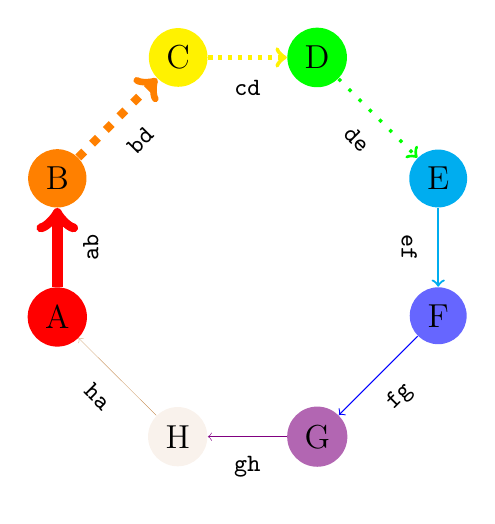
\begin{tikzpicture}[
    every node/.style = {font=\large, text=black, shape=circle},
    every edge/.style = {draw, ->},
    every edge quotes/.style = {below, font=\ttfamily\small,
      text=black, fill=none, sloped}]
  \node (a) [fill = red] {A};
  \node (b) [fill = orange,    above       = of a] {B};
  \node (c) [fill = yellow,    above right = of b] {C};
  \node (d) [fill = green,           right = of c] {D};
  \node (e) [fill = cyan,      below right = of d] {E};
  \node (f) [fill = blue!60,   below       = of e] {F};
  \node (g) [fill = violet!60, below left  = of f] {G};
  \node (h) [fill = brown!10,        left  = of g] {H};

  \draw (a) edge[line width=4pt, draw=red, "ab"] (b);
  \draw (b) edge[line width=3pt, draw=orange, loosely dotted, "bd"] (c);
  \draw (c) edge[ultra thick, draw=yellow, dotted, "cd"] (d);
  \draw (d) edge[very thick, draw=green, loosely dotted, "de"] (e);
  \draw (e) edge[thick, draw=cyan, "ef"] (f);
  \draw (f) edge[thin, draw=blue, "fg"] (g);
  \draw (g) edge[very thin, draw=violet, "gh"] (h);
  \draw (h) edge[ultra thin, draw=brown, "ha"] (a);
\end{tikzpicture}
\end{document}
